\documentclass[journal]{new-aiaa}
%\documentclass[conf]{new-aiaa} for conference papers
\usepackage[utf8]{inputenc}

\usepackage{graphicx}
\usepackage{amsmath}

\usepackage[version=4]{mhchem}
\usepackage{siunitx}
\usepackage{longtable,tabularx}
\setlength\LTleft{0pt}

\usepackage{amsmath}	% allows unnumbered equations with equation*
\usepackage{amssymb}	%% allows math logical symbols
\usepackage{graphicx}	% allows for graphics numbering

% Included by the user
\usepackage{fancyhdr}
\usepackage{afterpage}
\usepackage{float}		% allows to use [H] float, stricter version of [h]
\usepackage{matlab-prettifier}

\renewcommand{\headrulewidth}{0pt}
\pagestyle{fancy}
{
	\fancyhf{}
	\chead{Enrique Babio - Time Optimal Attitude Maneuvers}
	\cfoot{\thepage}
}
\fancypagestyle{fancyfirst}
{
	\fancyhf{}
	\chead{Enrique Babio}
	\cfoot{\thepage}
}

\title{Time-Optimal Attitude Maneuvers}
\author{ }

\begin{document}

\maketitle

\thispagestyle{fancyfirst}
\afterpage{\thispagestyle{fancy}}

\begin{abstract}
	The goal of this class project is to investigate the application of optimal control theory in attitude dynamics. In particular, we will focus on looking up time-optimal trajectories. Since there is no interest in any particular system, we use the dynamics for simple symmetric rigid-body. The problem of interest is to study the optimal control when the input consists of three controls acting on three orthogonal axis that where some norm of the control is bounded. The expected solution should be of bang-bang type. 
\end{abstract}

%\noindent(Nomenclature entries should have the units identified)

{\renewcommand\arraystretch{1.0}
	\noindent\begin{longtable*}{@{}l @{\quad=\quad} l@{}}
		$A$  & amplitude of oscillation \\
		$a$ &    cylinder diameter \\
		$C_p$& pressure coefficient \\
		$Cx$ & force coefficient in the \textit{x} direction \\
		$Cy$ & force coefficient in the \textit{y} direction \\
		c   & chord \\
		d$t$ & time step \\
		$Fx$ & $X$ component of the resultant pressure force acting on the vehicle \\
		$Fy$ & $Y$ component of the resultant pressure force acting on the vehicle \\
		$f, g$   & generic functions \\
		$h$  & height \\
		$i$  & time index during navigation \\
		$j$  & waypoint index \\
		$K$  & trailing-edge (TE) nondimensional angular deflection rate\\
		$\Theta$ & boundary-layer momentum thickness\\
		$\rho$ & density\\
		\multicolumn{2}{@{}l}{Subscripts}\\
		cg & center of gravity\\
		$G$ & generator body\\
		iso	& waypoint index
\end{longtable*}}

\section{Introduction}
Attitude maneuvers are a core problem to the control of aerospace vehicles. As such, understanding and optimizing the problem is a key aspect to the design of better performing vehicles. The performance index to be optimized will depend on the specific application and vehicle considered. For high performance aircraft and satellites, a possible performance index is the time used for a rest-to-rest maneuver. This has direct applications to satellite re-targeting or high-acceleration maneuvers for aircraft allowing for faster redirecting of the aircraft path. 

A survey on time-optimal maneuvers is provided by Scrivener \cite{scrivener1994survey}. Optimal maneuvers for different configurations: number of angular velocity controls, rigid and flexible bodies, and rotating around the eigenaxis are discussed.

Here, since we aim to achieve insight on maneuvers for both spacecraft and aircraft we will focus on rigid-body maneuvers under bounded controls. For large angle reorientations, introducing quaternions will simplify the problem of computing the difference between attitudes, besides avoiding the singularities of Euler angles, as proposed by Wie and Weiss \cite{wie1989quaternion}. In this case they introduce a regulator that follows the eigenaxis rotation between initial and final state which is the minimum action path. Chowdhry \cite{chowdhry1991optimal} solves the time-optimization of the attitude stabilization (i.e. drive angular velocity to 0) for different configurations where one angular rate control is not available for its application to super-maneuverable aircraft.

The problem is interesting from a theoretical point of view since it involves a number of different tools. The attitude equations of motion are highly nonlinear, and without any assumptions result in complex motion. Attitude itself calls for the use of quaternions or similar formulations since Euler angle strategies may become badly-defined and little intuitive. Finally, optimal control theory is necessary in order to achieve the necessary conditions for the time optimality of the control as stated by Longuski \cite{longuski2014optimal}. Besides, the final control is not readily intuitive: eigenaxis maneuvers provide the minimum length path, however aircraft tend to combine rolling and pitching motion.

In particular, we will follow the approach used by Bilimoria \cite{bilimoria1993time} and Fleming \cite{fleming2010minimum} but using a slightly different notation. An axis-symmetric rigid-body will be considered where all three angular velocities can be controlled independently and where the control is norm by some norm. It would also be interesting to follow some of the approaches used by Byers \cite{byers1993quasi} to look for real-time solving capabilities for the control so that it could be flyable.




\section{Analysis}

\subsection{Problem formulation}
As covered by Bilimoria the equations of motion for the rotation around principal axes of inertia are:
\begin{align}
I_x \dot{\Omega}_x + (I_z-I_y) \Omega_z \Omega_y &= \tau_x \\
I_y \dot{\Omega}_y + (I_x-I_z) \Omega_x \Omega_z &= \tau_y \\
I_z \dot{\Omega}_z + (I_y-I_x) \Omega_y \Omega_x &= \tau_z 
\end{align}

For simplicity, we will assume that the vehicle is symmetric and therefore all three moments of inertia are identical and equal to $I$. Under those conditions the equations of motion decouple into:
\begin{align}
I \dot{\Omega}_x &= \tau_x \\
I \dot{\Omega}_y &= \tau_y \\
I \dot{\Omega}_z &= \tau_z 
\end{align}

Or expressed in vector notation:
\begin{equation}
I \vec{\Omega} = \vec{\tau}
\end{equation}

And the control is bounded by:
\begin{equation}
|\tau_x|^q + |\tau_y|^q + |\tau_z|^q \leq \tau_{max}^q
\end{equation}

Where $q$ is the norm of interest; this is a general way of bounding the control.  The most interesting norms will be the 2-norm and the infinity-norm which correspond to a the maximum applied being independent of the direction and to three indepedently bounded controls by $\tau_{max}$.

We can consider all three controls to be equally bounded by $\tau_{max}$ we can non-dimensionalize the equations of motion using $u_i = \tau_i / \tau_{max}$ and a characteristic time $t=\sqrt{I / \tau_{max}}$ so the characteristic angular velocity $\omega_i = \Omega_i \sqrt{I / \tau_{max}}$. The vector equation of motion now simplifies to its final form:
\begin{equation}
\label{omegadot}
\vec{\omega} = \vec{u}
\end{equation}

Beside the equations relating velocity to the control torques we need the equations of motion for the attitude quaternions. A description on how quaternions relate to euler angles and angular velocities can be found in Parwana and Kothari\cite{parwana2017quaternion} and useful relations for quaternion derivatives are provided by Graf \cite{graf2008quaternions}. For more details on the quaternion convention or the derivation and partial differentiation we refer to the Appendix A. Our attitude quaternion is $q$ and we introduce a angular velocity quaternion $\omega = [0 \ \vec{\omega}]^T$
\begin{equation}
\label{qdot}
\dot{q} = 1/2  \ q \circ \omega
\end{equation}

Now we are ready to state our optimization problem. Our performance index is minimum final time, in other words:
\begin{equation}
\min J = t_f
\end{equation}
Subject to the vector process equations\ref{omegadot} and  \ref{qdot}. Our control by the definition of the non-dimensionalization is subject to $|u_i| \leq 1$. And the initial and final states are fixed and defined by the maneuver to be optimized:
\begin{align}
 q(0) &= \left[ 1 \quad 0 \quad 0 \quad 0 \right]^T \\
 q(t_f) &= q_f \\
 \vec{\omega}(0) &= \vec{\omega}(t_f) = 0
\end{align}

So the only free boundary is the final time $t_f$ which is the performance index to be minimized.

\subsection{Hamiltonian and costate equations}
With the formulation for the equations of motion we define the Hamiltonian for the motion:
\begin{equation}
H(x,u,\lambda) = \frac{1}{2} \lambda_q^T (q \circ \omega) + \lambda_\omega^T \vec{u}
\end{equation}

Where $\lambda_q$ and $\lambda_\omega$ are the co-state vectors with a size of 4 elements and 3 elements respectively. We realize that since there is no explicit time dependence the Hamiltonian is constant throughout the motion. 

In order to get the costate equations we get apply the Euler-Lagrange equations and find the appropiate derivatives. In order to simplify the resulting expressions Matrix calculus is used to come up with more compact expressions, see Appendix A for details on the derivation. The expression for the attitude costates is:
\begin{equation}
\label{lambdaqDot}
\dot{\lambda}_q = - \frac{\partial H}{\partial q} =  \frac{1}{2} \lambda_q \circ \omega
\end{equation}

The partial derivative for $\dot{\lambda}_\omega$ depends on omega which appears only in the quaternion product, but it cannot be obtained straight forward using the expressions for quaternion derivatives since $\dot{\lambda}_\omega$ is not a 4 element vector. However, if we extend it to a 4 element vector where the first element is forced to be 0 then we can find the partial derivative in terms of the imaginary part of the quaternion derivative.
\begin{equation}
\dot{\lambda}_\omega = - \frac{\partial H}{\partial \omega} = - \frac{1}{2} \text{Im}(q' \circ \lambda_q)
\end{equation}

The control logic is that of bang-bang controller which can be expected for a minimum-time type strategy. Because of this we have the possibility of having singular sub-arcs. Later we will have to study the possible consequences on the control.

We now look at the boundary conditions. In the problem statement we have stated that the final and initial states are fixed, also the initial time is fixed. Since the only free state is the final time $t_f$ we look for the associated condition in the transversality condition:
\begin{equation}
  H_f dt_f - \lambda^T dx_f + dg = H_f dt_f - \lambda^T dx_f + dt_f = (H_f + 1) dt_f \implies H_f + 1 = 0
\end{equation}

Since $dt_f$ is the only free differential. Also, since the Hamiltonian is constant we have that:
\begin{equation}
 H = -1
\end{equation}

\subsection{Derivation of the optimal control}

In order to find the optimal control we recognize that we have an inequality constraint in the control of the following form:
\begin{equation}
1 =  |u_x|^q + |u_y|^q + |u_z|^q
\end{equation}
This means that $H_u^*=0$ cannot be directly satisfied. This function is not a switching function either so we have to apply Pontryagin's Minimum Principle since in its most basic form. We have to look for the optimal control such that:
\begin{equation}
H(x^*, u^*, \lambda^*) \leq H(X^*, u, \lambda^*)
\end{equation}

Or equivalently for our Hamiltonian:
\begin{equation}
\lambda_\omega^{*T} \vec{u}^* \leq \lambda_\omega^{*T} \vec{u}
\end{equation}

Since the expression above is linear in terms of $\vec{u}$ the minimum will necessarily lie on the inequality constraint of the norm of $\vec{u}$. We introduce the constraint in the expression above by solving for $u_z$ in terms of $u_x$ and $u_y$ and the sign of $u_z$ which we don't know yet:
\begin{equation}
\label{uzFromNorm}
u_z = \text{sgn}(u_z) \ (1 - |u_x|^q - |u_y|^q)^{\frac{1}{q}}
\end{equation}

Now we have to look for a minimum of:
\begin{equation}
\label{unconstrainedOptimalControl}
\mathcal{L} = \lambda_{\omega_x} u_x + \lambda_{\omega_y} u_y + \text{sgn}(u_z) \lambda_{\omega_3} (1 - |u_x|^q - |u_y|^q)^{\frac{1}{q}}
\end{equation}

In order to find the minimum we take partial derivatives with respect $u_x$ and $u_y$. In the derivatives we identify the expression for $|u_z|$ so we substitute it back: 
\begin{align}
\label{partialLx}
\frac{\partial \mathcal{L}}{\partial u_x} &= 0 =\lambda_{\omega_x} - \text{sgn}(u_x u_z) \ \lambda_{\omega_z} \ (1 - |u_x|^q - |u_y|^q)^{\frac{1-q}{q}} |u_x|^{q-1} = \lambda_{\omega_x} - \text{sgn}(u_x u_z) \ \lambda_{\omega_z} \ |u_z|^{1-q} |u_x|^{q-1}\\
\label{partialLy}
\frac{\partial \mathcal{L}}{\partial u_y} &= 0 = \lambda_{\omega_y} - \text{sgn}(u_y u_z) \ \lambda_{\omega_z} \ (1 - |u_x|^q - |u_y|^q)^{\frac{1-q}{q}} |u_y|^{q-1} = \lambda_{\omega_y} - \text{sgn}(u_y u_z) \ \lambda_{\omega_z} \ |u_z|^{1-q} |u_y|^{q-1}
\end{align}

And on the expressions above we solve for $u_x$ or $u_y$:
\begin{align}
&\lambda_{\omega_{x,y}} - \text{sgn}(u_{x,y} u_z) \ \lambda_{\omega_z} \ |u_z|^{1-q} |u_{x,y}|^{q-1} = 0 \\
\implies &
\text{sgn}(u_{x,y}) |u_{x,y}|^{q-1} = \frac{\lambda_{\omega_{x,y}}}{\lambda_{\omega_z}} \text{sgn}(u_z) \ |u_z|^{q-1} \\
\implies &
\text{sgn}(u_{x,y}) |u_{x,y}| = \text{sgn}\left(\frac{\lambda_{\omega_{x,y}}}{\lambda_{\omega_z}}\right) \left|\frac{\lambda_{\omega_{x,y}}}{\lambda_{\omega_z}}\right|^{\frac{1}{q-1}}
 \text{sgn}(u_z) \ |u_z| \\
= &
\label{uxyFromuz}
u_{x,y} = \text{sgn}\left(\frac{\lambda_{\omega_{x,y}}}{\lambda_{\omega_z}}\right) \left|\frac{\lambda_{\omega_{x,y}}}{\lambda_{\omega_z}}\right|^{\frac{1}{q-1}}
u_z
\end{align}

And substituting these expressions in the expression we obtained in \ref{uzFromNorm} we obtain:
\begin{align}
& |u_z| = 
\left(
\frac{|u_z|^q}{|u_z|^q} \left|\frac{\lambda_{\omega_{z}}}{\lambda_{\omega_z}}\right|^{\frac{q}{q-1}}
|u_z|^q- \left|\frac{\lambda_{\omega_{x}}}{\lambda_{\omega_z}}\right|^{\frac{q}{q-1}}
|u_z|^q - \left|\frac{\lambda_{\omega_{x}}}{\lambda_{\omega_z}}\right|^{\frac{q}{q-1}}
|u_z|^q
\right)^{\frac{1}{q}} \\
\implies & 
|\lambda_{\omega_z}|^{\frac{q}{q-1}} = 
\frac{1}{|u_z|^q} |\lambda_{\omega_{z}}|^{\frac{q}{q-1}}
- |\lambda_{\omega_{x}}|^{\frac{q}{q-1}}
- |\lambda_{\omega_{x}}|^{\frac{q}{q-1}}
\\ \implies &
\frac{1}{|\lambda_{\omega_{z}}|^{\frac{q}{q-1}}}
|\lambda_{\omega_z}|^{\frac{q}{q-1}} + |\lambda_{\omega_{x}}|^{\frac{q}{q-1}}
+ |\lambda_{\omega_{x}}|^{\frac{q}{q-1}} = 
\frac{1}{|u_z|^q}
\\ \implies &
|u_z| = 
\frac{|\lambda_{\omega_{z}}|^{\frac{1}{q-1}}}
{\left[ |\lambda_{\omega_x}|^{\frac{q}{q-1}} + |\lambda_{\omega_y}|^{\frac{q}{q-1}} + |\lambda_{\omega_z}|^{\frac{q}{q-1}}\right]^\frac{1}{q}}
\end{align}

This defines the magnitude of each control input as function of the magnitude of the costates, but we still don't know how to find the sign of $u_z$. However to pick the right sign we just need to recall that our goal is to minimize the Hamiltonian, therefore we have to pick the sign with the opposite sign to $\lambda_{\omega_z}$. 

%% Legendre-Clebsch condition approach
\iffalse
In order to find it we make use of the Legendre-Clebsch condition on the unconstrained version of the problem we found on \ref{unconstrainedOptimalControl}. In \ref{partialLx}, \ref{partialLy} we found the first derivatives, in order to verify the Legendre-condition we take the second derivatives:
\begin{align}
\frac{\partial^2 \mathcal{L}}{{\partial u_x}^2} &=
-\text{sgn}(u_z) \ \lambda_{\omega_z} \ \left( -(1 - |u_x|^q - |u_y|^q)^{\frac{1-2q}{q}} |u_x|^{2q-2} + \ (1 - |u_x|^q - |u_y|^q)^{\frac{1-q}{q}} |u_x|^{q-2} \right) \\
&= -\text{sgn}(u_z) \ \lambda_{\omega_z} \ \left(-|u_z|^{1-2q} |u_x|^{2q-2} + |u_z|^{1-q} |u_x|^{q-2} \right) \nonumber
\\
\frac{\partial^2 \mathcal{L}}{{\partial u_y}^2} &= 
-\text{sgn}(u_z) \ \lambda_{\omega_z} \ \left( -(1 - |u_x|^q - |u_y|^q)^{\frac{1-2q}{q}} |u_y|^{2q-2} + \ (1 - |u_x|^q - |u_y|^q)^{\frac{1-q}{q}} |u_y|^{q-2} \right) \\
&= -\text{sgn}(u_z) \ \lambda_{\omega_z} \ \left(-|u_z|^{1-2q} |u_y|^{2q-2} + |u_z|^{1-q} |u_y|^{q-2} \right) \nonumber
\\
\frac{\partial^2 \mathcal{L}}{{\partial u_y}^2} &= 
\text{sgn}(u_z u_x u_y) \ \lambda_{\omega_z} \ \left( (1 - |u_x|^q - |u_y|^q)^{\frac{1-2q}{q}} |u_y|^{q-1} |u_x|^{q-1} \right) \\
&= \text{sgn}(u_z u_x u_y) \ \lambda_{\omega_z} \ |u_z|^{1-2q} |u_y|^{q-1} |u_x|^{q-1}
\end{align}
\fi

Once we have found the right $u_z$ we can solve for $u_{x,y}$, using \ref{uxyFromuz}. The expression for all three controls became similar as it could be expected:
\begin{equation}
\label{lqControl}
u_i = 
\frac{-\text{sgn}(\lambda_{\omega_{i}}) |\lambda_{\omega_{i}}|^{\frac{1}{q-1}}}
{\left[ |\lambda_{\omega_x}|^{\frac{q}{q-1}} + |\lambda_{\omega_y}|^{\frac{q}{q-1}} + |\lambda_{\omega_z}|^{\frac{q}{q-1}}\right]^\frac{1}{q}}
\end{equation}

Finally, we have to consider the possibility of singular control. In order to rule it out we recall the $H=-1$ condition obtained from the transversality condition. This allows us to guarantee that there will be non singular sub-arcs. Singular subarcs will only happen if $\lambda_\omega = 0$ for a finite interval, this implies that $\dot{\lambda}_\omega = 0$, but since $q$ is an atittude quaternion $\dot{\lambda}_\omega = 0$ will only happen if $\lambda_q=0$. This cannot happen at the same time that $\lambda_\omega = 0$ since that would make the Hamiltonian vanish, contradicting the transversality condition. Since there are no singular sub-arcs the controller above satisfies the necessary conditions for an optimal control. 

The controller structure is fundamentally of a bang-bang nature. There is a component controlling the allocation of the control to the different actuators, but on top of this amplitude allocation the sign is controlled in the same fashion as a usual bang-bang control. Choosing a norm will determine the behavior of the control amplitude allocation, allowing for more independence between the controls that will lead to more and more complex control profiles and possible faster maneuver since the set of possible controls increases with the norm. 

In the limit, where the norm goes to infinity the controls become completely independent with the form of switching functions. Each control component must satisfy $|u_i|\leq 1$. Then from the limit of the control in \ref{lqControl}, or following the usual reasoning for switching functions minimizing the Hamiltonian we get:
\begin{equation}
\label{lInfinityControl}
u_i = -\text{sgn}(\lambda_{\omega_{i}})
\end{equation}

\section{Numerical Solution}
Once the TPBVP has been defined, the next step is to solve it. The discussion of the numerical solution will be split in three different topics, the first one will discuss the general strategy used for the problem and the statement of the boundary conditions, the second one will cover the initial guesses used for the solver, the third one considers the possible methods used for the solution and the advantages and disadvantages of each one them.

\subsection{Statement of the constraints}
The problem to be solved right now can be thought of a feasibility problem where we satisfy the constraints of the TPBVP. As such we will resort to numerical methods for its solution, but we should try to reduce the dimensionality of the problem and improve its conditioning as much as possible.

The first guess for the numerical solver will be obtained from the numerical integration of some initial conditions. Since we know the initial values for the states these will be fixed and will not be allowed to change, this helps to reduce the dimensionality of the problem by 7 states. In the most basic form of the solution, we have reduced the problem to finding the initial values for the 7 co-states.

Also, we know that the Hamiltonian is constant throughout the motion and $H=-1$. The information that this constraint provides is merely in the terms of scaling of the costates. However, for our particular problem since the scaling of the co-states is not critical since we use them in two ways: for modulating amplitude (where the relative values is the used information) and for a switching function (where only the sign matters). This means that in order to avoid ill-conditioned numerical problems we can reformulate the constant Hamiltonian as:
\begin{equation}
|\lambda_{q_f}|=1
\end{equation}

But recalling the costate equation for $\dot{\lambda}_q$ we can observe that it is just the rotation in  time of $\lambda_q$ under the angular velocity $\vec{\omega}$. This means that the magnitude of $\lambda_q$ stays constant in time, and therefore we check the magnitude at the initial conditions where it is more convenient for our initial guess. Therefore the transversality condition is substituted by:
\begin{equation}
|\lambda_{q_0}|=1
\end{equation}

Other than this condition, we will also check for state constraints at the final time. Since the final time is variable it is also another variable to be found in our constraints feasibility problem solution. We have a total of 8 constraints, 7 states and the just found condition on the module of $\lambda_q$, and 8 free variables, the initial states and the final time, so the problem is well defined.

\subsection{Initial guesses and continuation strategy}
After defining the constraints to be satisfied, the next step is how to come up with initial guesses for the solver. All solvers will work by solving an approximated problem, therefore we must come up with an initial guess close enough to the final solution in order for the solver to converge.

A possible strategy is to use a continuation on the norm. If the solution for a specific norm is known, its initial co-states can be used as a first guess for the problem of a similar norm. However, in any case a initial solution for a particular norm must be known. In the followin paragraph we come up with an initial guess for the 2-norm controller, so for solving higher norm controllers we will continuate the norm up to our desired final norm.

In the case of the 2-norm control the initial solution can be found analytically with the following thought process. This solution is not meant to be a formal solution since it is only used as an initial guess. The 2-norm control has no preferred direction of control since all controls are embedded in a sphere, therefore the optimal control will be that uses the shortest path. This shortest path will correspond to the rotation about the eigenaxis that connects the initial and final states. Since the initial quaternion is fixed to $q_0=[1 \quad 0 \quad 0 \quad 0]^T$, the final quaternion provides the angle $\theta$ to be rotated and the eigenaxis $\vec{n}$ information in the angle-axis expression of the quaternion:
\begin{equation}
q(t) = \left( \cos \frac{\theta}{2} \ ,\ \sin\frac{\theta}{2} \ \vec{n} \right)
\end{equation}

In order to consider the time evolution of the rotation, we can consider the problem as a 1-d rotation where the rest-to-rest maneuver will follow a triangular angular velocity profile with one switch of the control exactly at the half of the path. The time to the switch since the beginning of the maneuver can be found as:
\begin{equation}
  \frac{1}{2} t_{sw} = \theta_f \quad \implies \quad t_f=2 t_{sw} = 2 \sqrt{\theta_f}
\end{equation}

The angular velocity must be parallel to the eigenaxis and therefore so will be the $\vec{u}$, the switching must happen in all three components at the same time and then they must be equal to zero at $t_f/2$. We previously said that $\lambda_q$ rotates in time with $\omega$ so it must follow also follow an eigenaxis rotation. We can express it as the composition of the rotation of $q$ and the initial offset:
\begin{equation}
\lambda_q = q(t) \lambda_{q_0}
\end{equation}

And then for $\lambda_\omega$ we get:
\begin{equation}
\dot{\lambda}_\omega = -\frac{1}{2} \text{Im}(q(t)' \circ q(t) \circ \lambda_{q_0}) = -\frac{1}{2} \text{Im}(\lambda_{q_0})
\end{equation}

So from the expression above states that $\lambda_{\omega}(t)$ is linear with time and knowing that $\lambda_{\omega}$ must be parallel to the rotation axis we can write the expression below. For that we use the fact that $\lambda_{\omega}(0)$ just oppose the rotation axis for the input to be aligned with it.
\begin{equation*}
\lambda_{\omega}(0) = \frac{1}{2} \text{Im}(\lambda_{q_0}) (t_f/2) = - k \vec{n}
\end{equation*}

So from this expression we get that:
\begin{align}
\lambda_{q_0} &= - [0 \quad \vec{n}]^T\\
\lambda_{\omega_0} &= -\frac{t_f}{4} \vec{n}
\end{align}

\subsection{Solving methods}
Different solvers for the feasibility problem were considered with their advantages and disadvantages. The options are summarized below with a discussion on their applicability to our problem of interest

\subsubsection{Collocation methods} 
They are based on discretization of the motion into several intervals where the motion is integrated usually in an implicit way. These methods are characterized by their efficiency but lack the accuracy of other methods. MATLAB's bvp4c was the first option to be tested since it is meant for this kind of problems. 

Its first problem comes from the collocation of swicthing and signum functions which cause the Jacobian to be singular. This was solved by approximating the signum function by a hyperbolic tangent so the continuation strategy would increase the norm and also the accuracy of the hyperbolic tangent approximation.

They are able to converge to valid solutions for low order norms but they were not able to converge with the desired accuracy as the continuation increased.

\subsubsection{Multiple shooting method with Newton Iterations}
A shooting method consists on running solving the feasibility problem by obtaining a Jacobian of how changes in the initial state about some guess change the final conditions. This is leads to a Newton iteration scheme where the errors and their Jacobian are used to compute the new initial conditions until the error is minimized.

The Jacobian approximation for changes in the initial conditions is only valid for an interval around the initial guess depending on the sensitivity of the problem. In order to minimize this sensitivity multiple shooting is used. It decreases the sensitivity by splitting the time interval into several intervals. On each of these intervals a shooting is performed. Since the number of states has increased, you have a initial state guess at the beginning of each shooting, extra constraints have to be added. These constraints ensure the continuity between shootings so that all different shootings are consistent. This decreases the sensitivity and increases the robustness of the method at the expense of more design constraints and increased computational cost. The preferred number of shooting intervals was set to 3.

In order to apply this method an integration scheme has to be used. Here MATLAB's ode 45 RungeKutta integrator was used with tight integration constraints to prevent numerical error from interfering in the computation of the Jacobian matrix. Specifically the relative tolerance was set to $10^{-11}$ and the absolute tolerance to $10^{-14}$.

This method works as long as the Jacobian approximation works. It seemed to have convergence problems as the norm increased. It may have been solved by decreasing the step in the continuation.

\subsubsection{Multiple shooting method with fmincon}
This method is based on the previous method. The integration and constraint formulation to ensure continuity between different shootings is formulated in the same way. The difference lies in the solver used to find the new initial guess after each iteration.

We used MATLAB's fmincon, a convex optimizer that allows for constraints directly. Therefore instead of trying to minimize the constraint functions in the way of an augmented Lagrangian objective function we let fmincon handle the constraints. This solver introduces methods for satisfying the constraint that go beyond the Newton's method we were using before. This leads to a greater radius of convergence.

The objective function to be minimized was time and the constraints were the ones already stated. However, we are not particularly interested in minimizing time, we already know that the solution will be time optimal if the constraints are satisfied. Optimization paramters are chosen according to this idea. The tolerance for the constraints is set to $10^{-4}$ and for the objective function optimility the tolerance is set to 1 since we are not really concerned about it.

This approach was the one that allowed for successful computation of the optimal control. The parameters for the integration are the same as those above. Results discussed below were found using this method.


\section{Results}

Results were obtained for an arbitrary maneuver. The initial state is neutral attitude: roll, pitch and yaw all equal to zero. The final state are the following roll, pitch and yaw angles (in that order):
\begin{equation}
\phi=-20^\circ \quad \theta=10^\circ \quad \psi=90^\circ
\end{equation}

We are particularly interested in two of the norms. The 2-norm and $\infty$-norm. The 2-norm shows the maneuver for the shortest path, can be computed in real time using the approximation provided in section IIIc, and works as a reference solution. The $\infty$-norm uses three independent bounds, resembles more closely the limits of an attitude control system, and offers the possibility for unexplored more optimal solutions than those found by the 2-norm.

We start by discussing in detail the solution for the 2-norm solution. Figure \ref{fig:l2Maneuver} shows the main characteristics of the maneuver. Time-history is provided for the main parameters of interest: the states, attitude (in Euler angles) and angular velocity, the applied torques and the co-states that the determine the input. The costates of the attitude are not represented since they do not offer any insight. The initial co-states for the maneuver are:
\begin{equation}
\lambda_{q_0} = [-0.0006 \quad 0.2474 \quad 0.0833 \quad -0.9532]^T \qquad
\lambda_{\omega_0} = [0.1583 \quad 0.0533 \quad -.6093]
\end{equation}

The total used for the maneuver is $2.5596$ and the amplitude of total rotated angle is $1.6378$ radians. A closer look to the graphics reveal that our initial guess for the solution is indeed correct. The $\lambda_{\omega}$ behave linearly with time and being equal to 0 at exactly the half of the motion where the inputs reverse. The amplitude of these is set so that they are aligned with the eigenaxis of the rotation.

\begin{figure}[h]
	\centering
	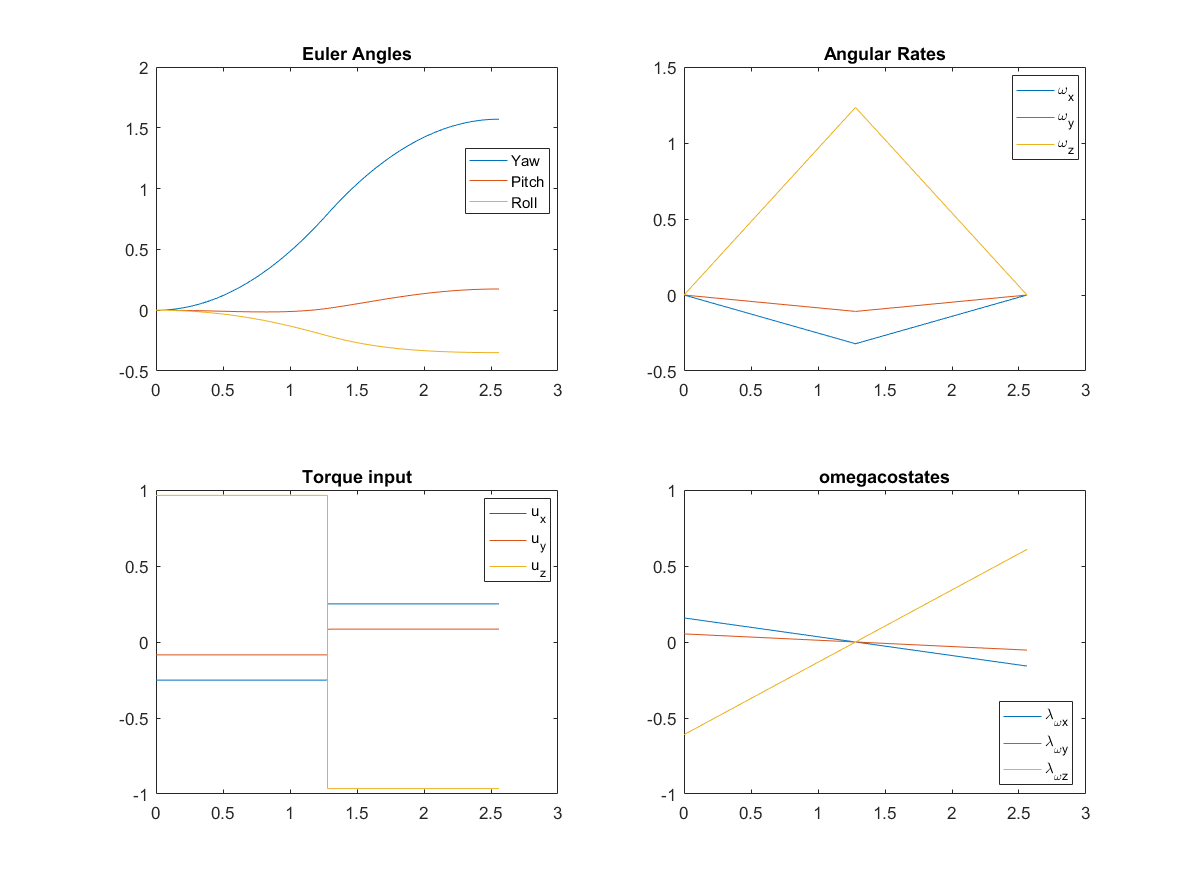
\includegraphics[height=12cm,keepaspectratio]{media/l2Maneuver.png}
	\caption{Solution, inputs and co-states for the switching function for the 2-norm optimal maneuver.}
	\label{fig:l2Maneuver}
\end{figure}

We now proceed to discuss the convergence process to the infinity norm. This was done by increasing the norm of the controller a about a 10 percent each iteration up to a norm of 20. Figure \ref{fig:lConvergence} shows some selected norms in the continuation process that show the evolution of the controller. As the norm of the controls increase the coupling between axes becomes more and more relaxed, for the $\infty$-norm they should be three independent controls bounds so the all three controls should lie on the $\pm1$ bound.

\begin{figure}
	\centering
	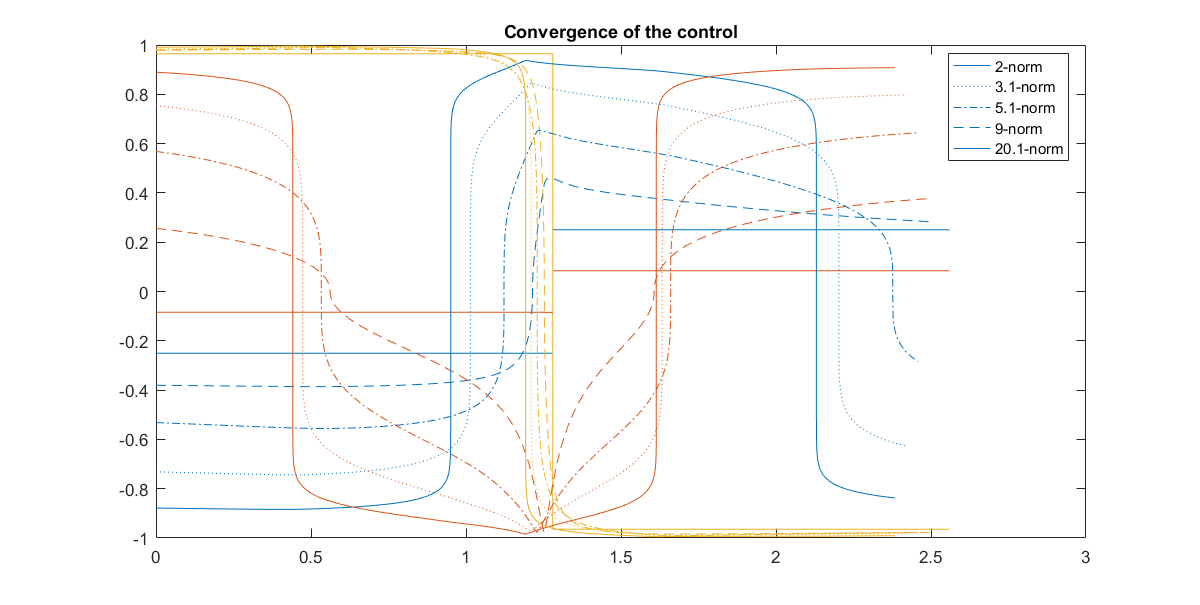
\includegraphics[height=8cm,keepaspectratio]{media/controlConvergence.png}
	\caption{Three axes controls for different norms ranging from to 2 to 20. As the norm increases the three controls become more and more decoupled. Reproduced from Bilimoria \cite{bilimoria1993time}.}
	\label{fig:lConvergence}
\end{figure}

Once the 20-norm controller is found, it is used as the starting solution for the $\infty$-norm controller implemented as in equation \ref{lInfinityControl}. The three controls become completely indepdent, the characteristics for the new control are plotted in figure \ref{fig:lInftyManeuver} in a similar fashion to those of the 2-norm control. The initial value for the co-states is:
\begin{equation}
\lambda_{q_0} = [-0.0405 \quad 0.0809 \quad -0.3818 \quad -0.9179]^T \qquad
\lambda_{\omega_0} = [0.0594 \quad -0.0751 \quad -.5617]
\end{equation}

The maneuver time has decreased to $2.3540$. A decrease above 8 percent in the maneuver time. The controls have the form of independent switching functions as it could be expected. This means that the angular velocity is also composed of linear intervals. These results are coherent with those found by Bilimoria$\cite{bilimoria1993time}$. The shape for the co-states of the switching function has become more complex.

It is interesting to note that the maneuver time has decreased with respect to the eigenaxis maneuver even though we are following a longer path. This is because the controller is reorienting the body so that a torque greater than any individual limit is applied in the desired rotation of motion from an inertial perspective as point out by Bilimoria\cite{bilimoria1993time}.

\begin{figure}[h]
	\centering
	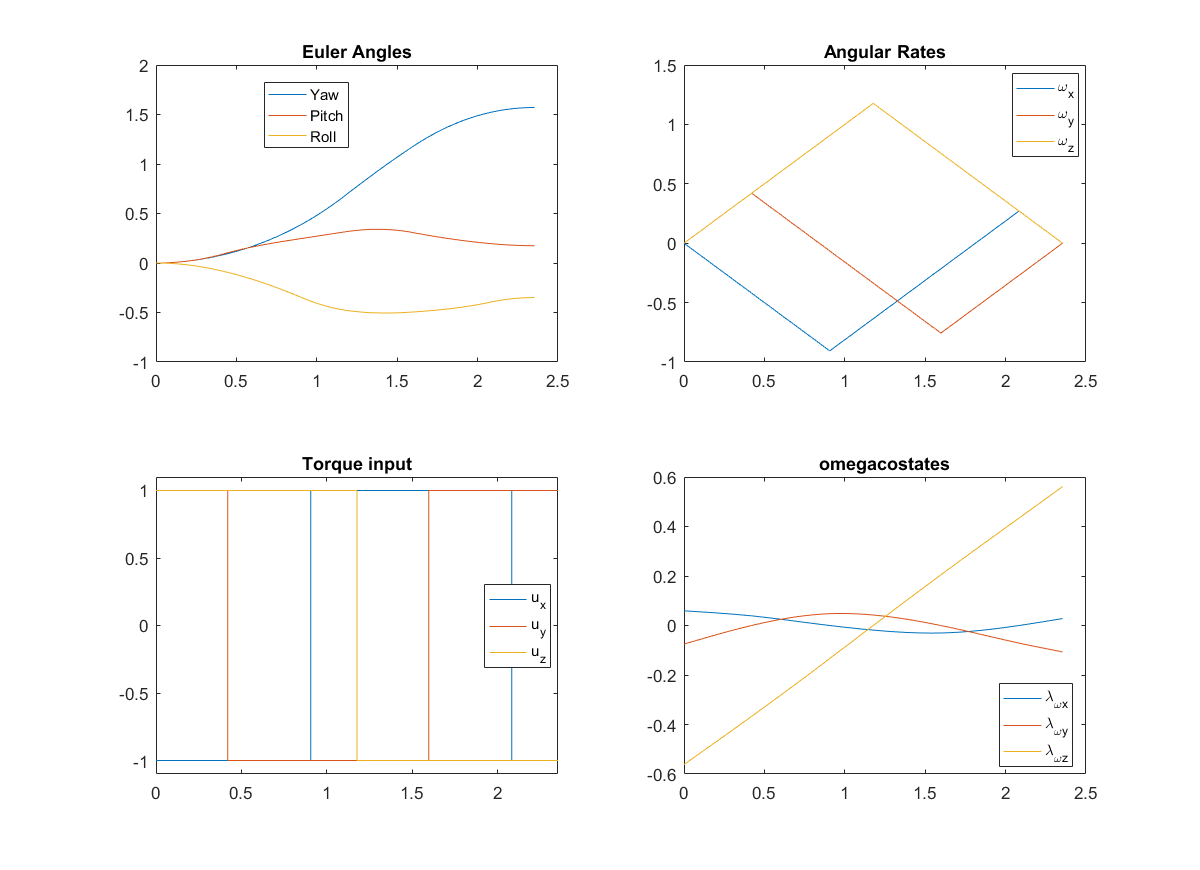
\includegraphics[height=12cm,keepaspectratio]{media/lInftyManeuver.png}
	\caption{Solution, inputs and costates for the switching function for the $\infty$-norm optimal maneuver.}
	\label{fig:lInftyManeuver}
\end{figure}

\section{Conclusions}
The time-optimal maneuver has been studied for the two most relevant cases: the 2-norm and the $\infty$-norm bounded controls. The conclusions from this work can be grouped in three main categories: optimality of the control, those regarding the solution, and finally the applicability and insight obtained from the results.

About the control we can state that:
\begin{enumerate}
	\item First order necessary conditions for an arbitrary norm control have been found using Pontryagin's Minimum Principle. The resulting control has the form of a modified switching function.
	
	\item For the $\infty$-norm controller, the resulting controls are independent switching functions.
	
	\item The existence of singular sub-arcs for the optimal solution has been ruled out.
	
	\item The trajectory between switches in the control can be solved analytically. A phase-space like approach could offer new insight.
\end{enumerate}

When it comes to solution of the system, the following can be concluded:
\begin{enumerate}
	\item The condition arising from the transversality condition can be rewritten to improve numerical conditioning in this particular problem.
	
	\item An analytical solution was found for the 2-norm controller or eigenaxis maneuver.
	
	\item A continuation strategy based on the norm can be used to find any specific norm. The $\infty$-norm was found following this procedure starting in the 2-norm.
	
	\item Multiple shooting methods can be used for increased robustness and accuracy in the solution at the expense of increased computation cost.
\end{enumerate}
	
Finally, about the method used and the results obtained we can state:

\begin{enumerate}
	\item Solutions of a norm higher than 2 improve the time used for a rest-to-rest attitude maneuver. In our particular example an improvement of 8\% was found.
	
	\item An arbitrary maneuver was tested. It has no special characteristics so this method should be applicable to any maneuver.
	
	\item The computation expense of the $\infty$-norm maneuver prevents it from its application to attitude control. The computation time used to find the initial co-states is not reasonable to be performed in real time. This can be done for 2-norm control since an analytical solution is known.
\end{enumerate}

This last finding is of critical importance to the applicability of this kind of maneuvers in real systems. Suboptimal approaches could be used to allow fast attitude maneuvers such as the 2-norm control. Other authors such as Byers\cite{byers1993quasi} have worked on this paper with intention of leveraging the known structure of the control to simplify the computations. As mentioned in the last point in the control related conclusions, a phase-space analysis may provide additional insight on this approach, and could lead into a global closed loop control, although the problem is likely to suffer from the curse of dimensionality.

Advances on the computational cost would allow the implementation of this kind of optimal maneuvers in the AOCS/FCS systems of spacecraft and aircraft. If the topic was to be researched more deeply the next steps would be in this direction.


\bibliography{aae508biblio}

\newpage
\appendix
\section*{Appendices}


\section{Mathematical notation}
\subsection{Quaternion and Vector notation and derivatives}
Here we use the so called Hamilton quaternion convention. A unitary quaternion $q$ with components $q_0, q_x, q_y, q_z$ is defined as:
\begin{equation}
 q = 
 \left[ \begin{matrix}
 q_0 & q_x & q_y & q_z
 \end{matrix}  \right]^T = \left( \cos \frac{\theta}{2} \ , \ \sin \frac{\theta}{2} \ \vec{n} \right)
\end{equation}
Where $q_0$ represents the real part of the quaternion associated with the rotation angle $\theta$ and $q_x, q_y, q_z$ represent the imaginary part associated with the rotation axis $\vec{n}$.

The quaternion product of the quaternions $q$ and $p$ is defined as usual and denoted by $q \circ p$. The quaternion conjugate is denoted by $q'$. We highlight the quaternion product as a matrix product as shown in Parwana \cite{parwana2017quaternion} and its relations with the conjugate quaternion:
\begin{equation}
q \circ p = (q' \circ p')' = Q(q) p = \bar{Q}(p) q 
= 
\left[\begin{matrix}
  q_0 & -q_x & -q_y & -q_z \\
  q_x & q_0 & -q_z & q_y \\
  q_y & q_z & q_0 & -q_x \\
  q_z & -q_y & q_x & q_0 
\end{matrix}\right]
 \left[ \begin{matrix}
p_0 \\ p_x \\ p_y \\ p_z
\end{matrix}  \right]
=
\left[\begin{matrix}
p_0 & -p_x & -p_y & -p_z \\
p_x & p_0 & p_z & -p_y \\
p_y & -p_z & p_0 & p_x \\
p_z & p_y & -p_x & p_0 
\end{matrix}\right]
\left[ \begin{matrix}
q_0 \\ q_x \\ q_y \\ q_z
\end{matrix}  \right]
\end{equation}

The time derivative of $q$ as a function of the angular velocity in the rotating body frame $\vec{\omega}$ is 
\begin{equation}
\dot{q} = 1/2  \ q \circ [0 \quad \vec{\omega}]^T
\end{equation}

In the Hamiltonian we get an expression of the form $\lambda^T (q \circ p)$, where $\lambda$ is a 4 element column vector. This expression is scalar. Expressing it as a matrix product we can find its derivative with respect to $q$ and $p$, using matrix calculus to obtain more compact expressions for the costates ODEs, we will use a column gradient convention. We start by finding the derivative of the quaternion product:
\begin{align}
\frac{\partial}{\partial p} \lambda^T (q \circ p) &= \frac{\partial}{\partial p} \lambda^T Q(q) p = (\lambda^T Q(q))^T = Q(q)^T \lambda = Q(q') \lambda = q'\circ \lambda \\
\frac{\partial}{\partial q} \lambda^T (q \circ p) &= \frac{\partial}{\partial p} \lambda^T \bar{Q}(p) q = (\lambda^T \bar{Q}(p))^T = \bar{Q}(p') \lambda = \lambda \circ p'
\end{align}

Where the derivative of the quaternion is obtained directly from Matrix calculus and the second one is obtained by inspection of the resulting matrix. We now obtain the expressions for the partial of the Hamiltonian taylored to the dynamics obtained for our problem:
\begin{equation}
H(x,u,\lambda) = \frac{1}{2} \lambda_q^T (q \circ \omega) + \lambda_\omega^T \vec{u}
\end{equation}

\begin{equation}
 - \frac{\partial H}{\partial q} = - \frac{1}{2} \frac{\partial}{\partial q}  \lambda_q^T (q \circ \omega) = - \frac{1}{2} \lambda_q \circ \omega' = \frac{1}{2} \lambda_q \circ \omega
\end{equation}
\begin{equation}
- \frac{\partial H}{\partial \omega} = - \frac{1}{2} \frac{\partial}{\partial \omega}  \lambda_q^T (q \circ \omega) = - \frac{1}{2} q' \circ \lambda_q
\end{equation}

\subsection{Derivative of a norm}
The norm used in this report is defined in terms of an absolute value for the greatest generality. We prove here the derivative:
\begin{equation}
\frac{d}{dx}|x|^q = 
\begin{cases}
\quad \frac{d}{dx}x^q = q \ x^{q-1} = q \ |x|^{q-1}\qquad &\text{for} \ x>0 \\
\quad \frac{d}{dx} (-x)^q = q \ (-x)^{q-1} =q \ |x|^{q-1} \qquad &\text{for} \ x<0 \\
\end{cases}
\end{equation}

Or in a more compact way using the signum function:
\begin{equation}
\frac{d}{dx}|x|^q = \text{sgn}(x) \ q \ |x|^{q-1}
\end{equation}

We will also use extensively the following property of the signum function:
\begin{equation}
\text{sgn}(x \ y) = \text{sgn}(x) \ \text{sgn}(y)
\end{equation}

\newpage
\input{textfiles/appendixCode}




\end{document}